\chapter{Wyniki Symulacji Wyspy Królików}
\label{app:wynikiSymulacjiWyspyKrolikow}

\par W ramach procesu testowania aplikacji postanowiono wykorzystać symulację "Wyspy Królików" (więcej informacji można znaleźć w sekcji \ref{subsec:rabbitIslandSimulation}). Symulacja ta zawiera następujące parametry wejściowe:

\begin{center}
	\texttt{
		\begin{tabular}{|c | c | c |}
			\hline
			Nazwa Parametru & Typ & Przyjęta Wartość \\
			\hline
			\hline
			RabbitsInitialPopulation & long & Zmienna w zależności od testu \\
			\hline
			RabbitsMinChildren & long & 0 \\
			\hline
			RabbitsMaxChildren & long & 6 \\
			\hline
			RabbitsPregnancyDuration & long & 2 \\
			\hline
			RabbitsLifeExpectancy & long & 6 \\
			\hline
			WolvesInitialPopulation & long & Zmienna w zależności od testu \\
			\hline
			WolvesMinChildren & long & 0 \\
			\hline
			WolvesMaxChildren & long & 6 \\
			\hline
			WolvesPregnancyDuration & long & 4 \\
			\hline
			WolvesLifeExpectancy & long & 14 \\
			\hline
			TimeRate & long & 3600 \\
			\hline
			DeathFromOldAge & boolean & true \\
			\hline
			MaxCreatures & long & 500 \\
			\hline
			FruitsPerDay & long & 60 \\
			\hline
			MapSize & long & 500 \\
			\hline
			MutationChance & double & 0 \\
			\hline
			MutationImpact & double & 0 \\
			\hline
			OffspringGenerationMethod & long & 0 \\
			\hline
			Timeout & long & 600 \\
			\hline
		\end{tabular}
	}
\end{center}

Wartymi szczególnej uwagi są tutaj:
\begin{itemize}
	\item \texttt{MaxCreatures} - określa maksymalną ilość stworzeń symulowanych w tym samym czasie.
	\item \texttt{TimeRate} - parametr ten decyduje o ile razy szybciej będą działy się wydarzenia w symulacji niż w rzeczywistości. W naszym przypadku przyjmuje on wartość \emph{3600}, co oznacza, że \emph{1} sekunda czasu rzeczywistego to \emph{1} godzina czasu symulowanego.
	\item \texttt{DeathFromOldAge} - jeżeli ustawiony na wartość \texttt{true}, to wartości \texttt{RabbitsLifeExpectancy} i \texttt{WolvesLifeExpectancy} są brane pod uwagę i kreatury umierają nie tylko w wyniku obrażeń, ale i ze starości.
	\item \texttt{Timeout} - określa po jakim czasie (wyrażonym w sekundach czasu rzeczywistego) symulacja ma zostać przerwana.
\end{itemize}

Natomiast za pomocą \texttt{RabbitsInitialPopulation} i \texttt{WolvesInitialPopulation} będziemy sterować początkowymi populacjami ssaków na wyspie. Symulacja kończy się w momencie wymarcia wszystkich kreatur lub przekroczeniu czasu \texttt{Timeout}.

\subsection{Test 1: Zerowa populacja królików}

\par W przypadku pierwszego testu, postanowiona sprawdzić czy założenia symulacji pokryją się z otrzymanymi wynikami. Przy zerowej populacji królików, wszystkie wilki powinny po pewnym czasie wymrzeć z głodu. Sukces tego testu możemy zaobserwować na grafie \ref{fig:rabbitIslandTest1Diagram1}, który powstał na bazie otrzymanych wyników. Początkową populację ustawiono na \emph{14}.

\begin{figure}
	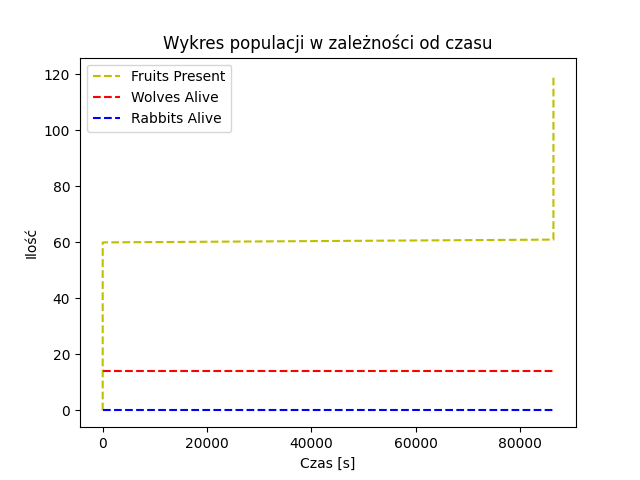
\includegraphics{RabbitIsland - Test 1}
	\caption{Wyspa Królików - Test 1 Diagram}
	\source{Opracowanie własne.}
	\label{fig:rabbitIslandTest1Diagram1}
\end{figure}

\subsection{Test 2: Zerowa populacja wilków}

\par Drugi test sprawdza sytuację analogiczną do pierwszej, tym razem jednak z królikami w roli głównej. Ilość stworzeń na start ustawiono na \emph{14}. Przewidywane są dwa poprawne rezultaty:
\begin{itemize}
	\item Populacja królików urośnie do takiego stopnia, że przychód nowych owoców nie będzie w staniej jej utrzymać. Następnie zacznie się nagłe wymieranie, spowodowane niedostatkiem pokarmu.
	\item Zostanie osiągnięty pewien poziom, na którym populacja królików ustabilizuje się.
\end{itemize}

\begin{figure}
	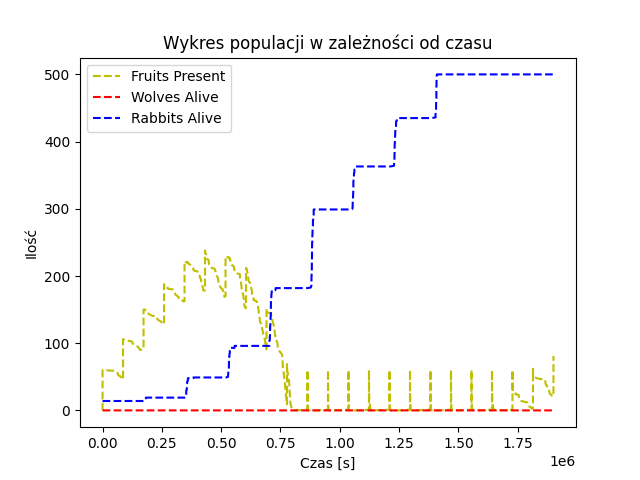
\includegraphics{RabbitIsland - Test 2}
	\caption{Wyspa Królików - Test 2 Diagram}
	\source{Opracowanie własne.}
	\label{fig:rabbitIslandTest2Diagram1}
\end{figure}

\par Na bazie otrzymanego wyniku (grafika \ref{fig:rabbitIslandSecondTestDiagramOne}), możemy stwierdzić, że spełnił się drugi z przewidywanych scenariuszy, jednak nie ze względu na naturalną stabilizację, ale twardy limit stworzeń, ustawiony przez jeden z parametrów. Okresem wzbudzającym zainteresowanie, jest pierwsze kilka dni, gdzie widzimy, jak gromadzi się nadmiar owoców. Ilość owoców osiągnęła swoje globalne maksimum na początku piątego dnia. Rezultaty tego dostatku, możemy zaobserwować w następnych dniach, gdzie występują największe przyrosty populacji królików (koreluje to z ustawionym czasem trwania ciąży - \emph{2 dni}).

\subsection{Test 3: Mieszanie wilków z królikami}

\par Ostatni z wykonanych testów miał za zadanie sprawdzić interakcję pomiędzy dwoma typami stworzeń. Początkowe populacje zostały ustawione na \emph{14} wilków i \emph{24} króliki. Wszystkie pozostałe parametry pozostały bez zmian.

\par Z otrzymanych rezultatów (grafiki \ref{fig:rabbitIslandTest3Diagram1} i \ref{fig:rabbitIslandTest3Diagram2}) możemy wywnioskować, że takie dobranie populacji było nietrafione. Ze względu na stosunkowo nieduży rozmiar mapy, jak i dużą ilość drapieżników populacja królików szybko zmalała do pojedynczego przedstawiciela tego gatunku. Co z kolei spowodowało iż owoce zaczęły się gromadzić, jak i doprowadziło finalnie populację wilków do wymarcia z powodu głodu.

\begin{figure}[H]
	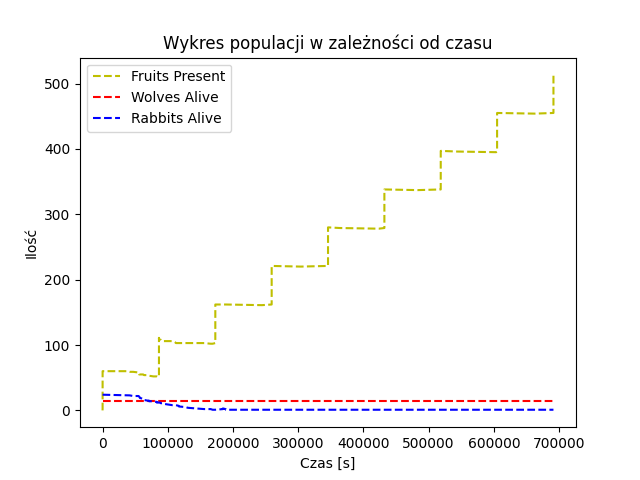
\includegraphics{RabbitIsland - Test 3 1}
	\caption{Wyspa Królików - Test 3 Diagram 1 - Wszystkie populacje}
	\source{Opracowanie własne.}
	\label{fig:rabbitIslandTest3Diagram1}
\end{figure}

\begin{figure}[H]
	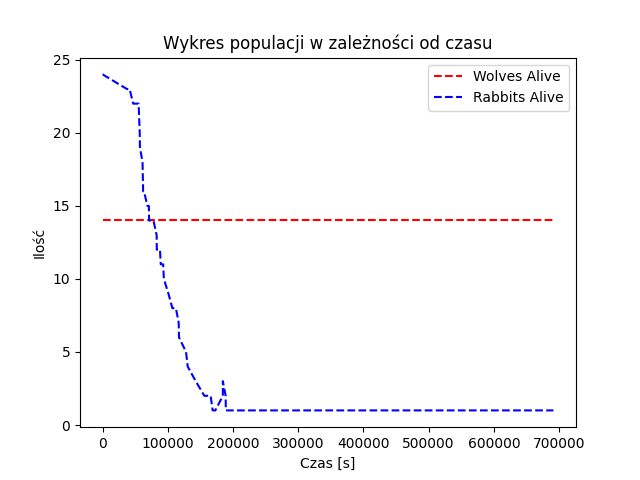
\includegraphics{RabbitIsland - Test 3 2}
	\caption{Wyspa Królików - Test 3 Diagram 2 - Ukryta ilość owoców }
	\source{Opracowanie własne.}
	\label{fig:rabbitIslandTest3Diagram2}
\end{figure}
